\documentclass{article}
\usepackage[letterpaper, total={6.75in, 9in}]{geometry} % good with line numbers
%\usepackage[top=0.5in,bottom=0.5in,left=0.5in,right=0.5in]{geometry} % Reduce the size of the margin to save paper
\usepackage{booktabs}
\usepackage{graphicx}
\usepackage{xurl} % permit line breaks in urls
\usepackage[luatex,plainpages=false]{hyperref}
\usepackage{lineno}
\usepackage{datetime2}
\usepackage{breakcites} % allow citatation to wrap
\usepackage{makeidx}         % allows index generation
\usepackage[utf8]{inputenc}
%\usepackage{setspace} \doublespacing
%\doublespacing % turn on doublespacing for the whole document.
\usepackage{parskip} % add a blank line between paragraphs upon export to PDF.
\usepackage[T1]{fontenc}
\usepackage{authblk}
\usepackage[labelfont=bf]{caption}
\DeclareCaptionType{equ}[][] % provide equ environment to add captions to equations
\usepackage[bottom]{footmisc}% places footnotes at page bottom
\usepackage{amsfonts, mathtools, amssymb, amssymb} % For math fonts, symbols and environments
\usepackage{booktabs} % Needed for fancy tables
\usepackage{threeparttable}
\usepackage{graphicx}
\usepackage{wrapfig} % Allows in-line images
\usepackage[labelfont=bf]{caption} % Make figure numbering in captions bold
% \usepackage{minted} invoke -shell-escape flag
%Print page numbers in the upper right corner rather than the bottom center.
\pagestyle{myheadings}
\usepackage{lastpage}
\usepackage{fancyhdr}
\pagestyle{fancy}
\fancyhf{} % Clear all header and footer fields
\fancyhead[L]{\today}
\fancyhead[C]{0573 Crystal detection} % Center header
\fancyhead[R]{\thepage\ / \pageref{LastPage}} 

% Three glossaries, the order matters here
\usepackage[acronym]{glossaries}
\newglossary[nlg]{notation}{not}{ntn}{Notation}
\makeglossaries
\setacronymstyle{long-short}
\loadglsentries{glossaries/acronyms}
\loadglsentries{glossaries/glossary}
\loadglsentries{glossaries/notation}

%backmatter
\bibliographystyle{cell}
\makeindex
% The following command produces a single column author index.
\RequirePackage{authorindex}
% Use this, if you want hyperlinks back from list of author entry to page
% where the citation was placed
\def\theaipage{\string\hyperpage{\thepage}} 
\newcommand{\listofauthorsname}{List of Authors}%
\newcommand{\listofauthors}% {%\section*{\listofauthorsname}%
% %\begin{multicols*}{2}
% \phantomsection%
% \addcontentsline{toc}{chapter}{\listofauthorsname}%
% \noindent%
\printauthorindex%
% Set the depth of the table of contents
\setcounter{tocdepth}{2} % 1 for sections, 2 for subsections, 3 for subsubsections, etc.

% Rename Reference section
\renewcommand{\refname}{Literature Cite}

% Create a code float environment to enclosed minted environments so that captions can be added to code listings.
\newenvironment{code}{\captionsetup{type=listing}}{}
% Approximate Arial font. To save ink by returning to a sans serif font, comment the next two lines.
\usepackage{helvet}
\renewcommand{\familydefault}{\sfdefault}
\modulolinenumbers[1]
\setlength{\parindent}{0pt} % Remove automatic indent of paragraphs.


\author[1]{Graduate Student}
\author[2]{Senior Collaborator}
\author[3]{Staff Scientist}
\author[1,2,3]{Blaine Mooers\thanks{blaine-mooers at ouhsc.edu, phone: 405-271-8XXX, FAX: 405-271-3X3X}}
\affil[1]{Department of Biochemistry and Molecular Biology, University of Oklahoma Health Sciences Center, Oklahoma City, Oklahoma, United States 73104}
\affil[2]{Stephenson Cancer Center, University of Oklahoma Health Sciences Center, Oklahoma City, Oklahoma, United States 73104}
\affil[3]{Laboratory of Biomolecular Structure and Function, University of Oklahoma Health Sciences Center, Oklahoma City, Oklahoma, United States 73104}


\title{An\gls{annotated bibliography}: Molecular graphics}

\usepackage{bibentry}
\nobibliography*

\begin{document}
\maketitle
\tableofcontents

% If the sections are unnumbered, they are invisible to the table of contents unless you use the addcontentsline command.
\section*{Illustrated and annotated bibliography}
\addcontentsline{toc}{section}{Illustrated and annotated bibliography}

\subsection*{\bibentry{Mooers2020ShortcutsForFasterImageCreationInPyMOL}}
\addcontentsline{toc}{subsection}{Mooers2020ShortcutsForFasterImageCreationInPyMOL}
%!TEX root = /Users/blaine/0573CrystalDetectionMeasurement/abibtests/inputNotesBibTeX/abib0537.tex

% Mooers2020ShortcutsForFasterImageCreationInPyMOL.tex

\subsubsection*{Summary} 
PyMOL is a tool for generating images of biomolecular structures, offering extensive control over their appearance through numerous parameters. \index{PyMOL}
To enhance and simplify its use, 241 Python functions, termed “shortcuts,” were developed. \index{Python}
These shortcuts, organized into 25 functional groups, allow users to perform tasks such as creating new molecular representations, saving files with unique time-stamped names, and conducting web searches directly from PyMOL. \index{molecular representaton}

\subsubsection*{Context in Molecular Graphics and Human-Computer Interactions} 
To streamline and enhance user interactions with PyMOL, 241 Python functions, known as “shortcuts,” were developed.\index{shortcuts} 
These shortcuts, categorized into 25 functional groups, facilitate tasks such as creating innovative molecular representations, saving files with unique time-stamped names to prevent overwriting, and conducting web searches directly from PyMOL. 
The help function provides documentation and reusable PyMOL commands, significantly improving user efficiency by reducing the time spent searching for code fragments.\index{code reuse}  
This integration of shortcuts exemplifies the synergy between molecular graphics and user-friendly interfaces, optimizing the workflow for researchers and scientists.
This is an excellent of good \gls{hci} \index{human-computer interactions}.

\subsection*{\bibentry{Mooers2021TemplatesForWritingPyMOLScripts}}
\addcontentsline{toc}{subsection}{Mooers2021TemplatesForWritingPyMOLScripts}
% Mooers2021TemplatesNotes

\subsubsection*{Summary}
PyMOL commands offer precise control over the visualization of molecular models, making PyMOL a favored tool for creating images of protein structures for publications and presentations. However, many users struggle to remember these commands due to infrequent use, complicating writing new scripts. 
One practical approach to address this issue is using code fragments as templates for different parts of the task. 
These fragments can be accessed from a library while coding in text editors like Visual Studio Code, Vim, and Emacs.


To facilitate this, we developed a library of PyMOL code templates, known as pymolsnips, which simplifies the process of writing PyMOL scripts. 
Pymolsnips is available on GitHub in formats compatible with 18 popular text editors, supporting Mac, Windows, and Linux operating systems. 
The GitHub repository also includes animations to guide users through the installation process for each text editor. 
This library will significantly enhance the productivity of PyMOL users when scripting.


\subsubsection*{Context in Molecular Graphics and Human-Computer Interaction}
\begin{wrapfigure}{l}{0.35\textwidth} % Example figure with text wrapping around it
\vspace{-10pt}
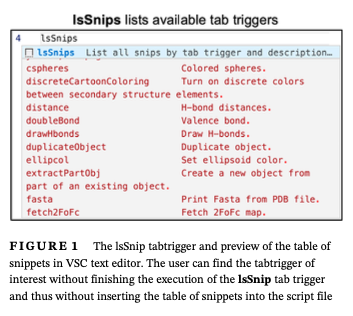
\includegraphics[scale=0.4]{imagesBlaine/Mooers2021TemplatesFig1.png}
\caption{\footnotesize Text wrapped image }
\vspace{-10pt}
\label{fig:preview}
\end{wrapfigure}

Tools like PyMOL and libraries like pymolsnips play a crucial role in the broader context of molecular graphics and human-computer interaction. 
Molecular graphics software allows scientists to visualize complex molecular structures, aiding in the understanding and communicating biochemical processes. 
The ability to precisely control these visualizations is essential for producing high-quality images for research and educational purposes.


Human-computer interaction (HCI) principles are integral to the design of these tools, ensuring they are user-friendly and accessible.
Visual Studio Code provide excellent usr interface to snippets (See Fig \ref{fig:preview}). 
By providing code snippets and templates, pymolsnips enhances the usability of PyMOL, making it easier for users to create and modify scripts without needing to recall specific commands. 
This approach aligns with HCI goals of improving efficiency and reducing cognitive load, ultimately fostering a more productive and intuitive user experience.

\subsubsection*{Snippet interfaces in Text Editors}


\begin{table}[ht]
\begin{center}
\caption{Tools by target skill level.}
\begin{tabular}{l c c c c}
\toprule
\multicolumn{1}{l}{\bf{Skill level}} & {\bf{Shortcuts}} & {\bf{Snippets}} & {\bf{Polyglot docs}} & {\bf{Quizzes}}\\
\midrule
Beginner        &  \checkmark  &           &             &  \checkmark  \\
Adv. Beginner   &  \checkmark & \checkmark &             &   \checkmark  \\
Competent       &  \checkmark & \checkmark &  \checkmark &   \checkmark  \\
Proficient.     &  \checkmark & \checkmark &  \checkmark &   \checkmark   \\
Expert          &  \checkmark & \checkmark &  \checkmark &   \checkmark   \\
\hline 
\end{tabular}
\label{tab:skilllevel}
\end{center}
\end{table}

Pymolsnips can be used at all skill levels (Table \ref{tab:skilllevel}).
PyMOL users can be divided into five levels of skill \cite{Dreyfus1980AFiveStageModelOfTheMentalActivitiesInvolvedInDirectedSkillAcquisition}. 
Beginner users may represent ~40\% of PyMOL users (Table 1). 
Their use of PyMOL is generally limited to viewing and comparing structures.
Beginner users are not yet willing to invest in learning the commands of the PyMOL macro language. 
They prefer the intuitive nature of the PyMOL GUI and its pulldown menus. 

Advanced beginners (~30\% of users) are able to navigate the GUI quickly. 
They also use simple commands like the ``fetch'' command to retrieve coordinate files from the Protein Data Bank. 
They may make images of global views and structure superpositions. 
They also make simple close-up views of protein-ligand interactions and subunit-subunit interfaces. 
They rely on session files to save work in progress. 
Competent users (~20\% of users) use scripts to assemble images for publication.
Proficient users (~9\% of users) know most of the frequently used parameters and are willing to invest time in learning new commands. 
They have been using text editors for years but may not have discovered the power of snippet libraries. 

The expert users (~1\%) understand the PyMOL macro language syntax and remember many of the commands. 
They extend the capability of PyMOL by importing functions from modules outside of PyMOL.
They may even be involved in the development of new plugins. 
They are likely expert users of one or more text editors. 
They would welcome a snippet library and the shortcuts. 
The tools developed in this proposal will benefit users at all levels of expertise and help them to move to higher levels of expertise (Table 1).


% % You have to tweak the textwidth to move the caption to the right to align with the table.
% \begin{wraptable}{r}{0.60\textwidth} % Example table with text wrapping around it
% \caption{Tools by target skill level.}
% \begin{center}
% \vspace{-20pt}
% \begin{threeparttable}
% \begin{tabular}{l c c c c}
% \toprule
% \multicolumn{1}{l}{\bf{Skill level}} & {\bf{Shortcuts}} & {\bf{Snippets}} & {\bf{Polyglot docs}} & {\bf{Quizzes}}\\
% \midrule
% Beginner        &  \checkmark  &           &             &  \checkmark  \\
% Adv. Beginner   &  \checkmark & \checkmark &             &   \checkmark  \\
% Competent       &  \checkmark & \checkmark &  \checkmark &   \checkmark  \\
% Proficient.     &  \checkmark & \checkmark &  \checkmark &   \checkmark   \\
% Expert          &  \checkmark & \checkmark &  \checkmark &   \checkmark   \\
% \hline
% \end{tabular}
% \end{threeparttable}
% %\footnotesize\textsuperscript{a}{All participants clowns.}
% \vspace{-10pt}
% \end{center}
% \label{tab:skilllevel}
% \end{wraptable}



\newpage
\addcontentsline{toc}{section}{Acronyms}
\printglossary[type=\acronymtype] % Print the acronym list
\clearpage
\addcontentsline{toc}{section}{Glossary}
\printglossary % Print the main glossary
\clearpage
\addcontentsline{toc}{section}{Mathematical Notation}
\glsaddall[types={notation}] % add all entries, not just those used.
\printglossary[type=notation, title=Mathematical Notation]
\addcontentsline{toc}{section}{Literature Cited}
\bibliography{mabib0573}
\addcontentsline{toc}{section}{Index}
\printindex
%\listofauthors  
\end{document}